% ****** Start of file apssamp.tex ******
%
%   This file is part of the APS files in the REVTeX 4.2 distribution.
%   Version 4.2a of REVTeX, December 2014
%
%   Copyright (c) 2014 The American Physical Society.
%
%   See the REVTeX 4 README file for restrictions and more information.
%
% TeX'ing this file requires that you have AMS-LaTeX 2.0 installed
% as well as the rest of the prerequisites for REVTeX 4.2
%
% See the REVTeX 4 README file
% It also requires running BibTeX. The commands are as follows:
%
%  1)  latex apssamp.tex
%  2)  bibtex apssamp
%  3)  latex apssamp.tex
%  4)  latex apssamp.tex
%
\documentclass[%
 reprint,
%superscriptaddress,
%groupedaddress,
%unsortedaddress,
%runinaddress,
%frontmatterverbose,
%preprint,
%preprintnumbers,
%nofootinbib,
%nobibnotes,
%bibnotes,
 amsmath,amssymb,
 aps,
%pra,
%prb,
%rmp,
%prstab,
%prstper,
%floatfix,
]{revtex4-2}

\usepackage{graphicx}% Include figure files
\usepackage{dcolumn}% Align table columns on decimal point
\usepackage{bm}% bold math
%\usepackage{hyperref}% add hypertext capabilities
%\usepackage[mathlines]{lineno}% Enable numbering of text and display math
%\linenumbers\relax % Commence numbering lines
\usepackage{tikz}
\usepackage[compat=1.1.0]{tikz-feynman}

%\usepackage[showframe,%Uncomment any one of the following lines to test
%%scale=0.7, marginratio={1:1, 2:3}, ignoreall,% default settings
%%text={7in,10in},centering,
%%margin=1.5in,
%%total={6.5in,8.75in}, top=1.2in, left=0.9in, includefoot,
%%height=10in,a5paper,hmargin={3cm,0.8in},
%]{geometry}

\begin{document}

% \preprint{APS/123-QED}

\title{Determination of cross sections for $pp \rightarrow Z \rightarrow ee$ using 13 TeV ATLAS open data}
% \thanks{A footnote to the article title}

\author{Ben Gavan\\10301715}
\affiliation{%
School of Physics \& Astronomy\\
University of Manchester
}
% \altaffiliation[Also at ]{Physics Department, XYZ University.}%Lines break automatically or can be forced with \\


%  \collaboration{MUSO Collaboration}%\noaffiliation


\date{\today}% It is always \today, today,
%  but any date may be explicitly specified

\begin{abstract}
The cross section of $Z \rightarrow e^{+}e^{-}$ was determined using the 13 TeV ATLAS open data set by comparing experimental data and Monte Carlo simulations to motivate selection cuts in an attempt to isolate possible signal events. By varying these selection cuts, an estimation of the systematic uncertainty was made. The cross section, $\sigma$, for $Z \rightarrow e^{+}e^{-}$ was calculated to be {$\sigma (pp \rightarrow Z \rightarrow ) = 1.988\pm0.001 (\text{stat.}) \pm 0.136 (\text{syst.}) \pm 0.0338 (\text{lumi.}) \text{ nb}$}. These values are consistent with accepted values.
\end{abstract}

\maketitle

%%%%%%%%%%%%%%%%%%%%%%%%%%%%%%%%%% Introduction %%%%%%%%%%%%%%%%%%%%%%%%%%%%%%%%%%
\section{Introduction}
To determine the cross section of the Z boson decay mode $Z \rightarrow e^{+}e^{-}$ the 13 TeV ATLAS open data set was used. Four main steps were taken to complete this: 1) Apply basic cuts using physical motivations, 2) Plot key kinematic variables to motivate/find further cuts. 3) Calculate cross section for process. 4) Estimate systematic uncertainties.
% \section{Background}

% \subsection{The ATLAS Experiment}
% The ATLAS experiment is located at one of beam collision points at the LHC. 

% \subsection{Monte Carlo Simulation}
% Monte Carlo simulations are used to make predictions of experimental observables at ATLAS 
% % To generate the simulated data, Monte Carlo simulations are used.  
%%%%%%%%%%%%%%%%%%%%%%%%%%%%%%%%%% Theory %%%%%%%%%%%%%%%%%%%%%%%%%%%%%%%%%%
\section{Theory}
Using the LHC, bunches of protons are accelerated and collided at cross over points. When two bunches cross, there is a probability protons can collide.  When they collide, many particles are produced. Due to the magnetic field produced by the magnetic solenoid, low rest mass charged particles are made to spiral, resulting in only high transverse momentum particles passing through the detector in relatively straight lines.  For example, the Z boson is produced close to rest and when it decays by the most common mode, the two products will be produced back to back with large transverse momentum. A jet can also be produced which would cause the lepton pair to be boosted and have a decreased azimuthal angle between them.

The ATLAS detector reconstructs interesting events in terms of individual particle candidates.  The main kinematic variables used in this analysis are: transverse momenta ($p_T$), azimuthal angle ($\phi$), pseudorapidity ($\eta$) and the isolation variables ptcone30 and etcone20. The isolation variables ptcone30 and etcon20 are measures of how isolated a detected lepton candidate is. A completely isolated lepton is one where there is no other sources of signal in a cone around the lepton with the apex at the reconstructed production origin.  Therefore \textit{ptcone30} is the sum of transverse momenta of all tracks detected within a cone of  $\Delta R = 0.3$ excluding the lepton itself. \cite{opendata-atlas}. $\Delta R$ is defined as 
\begin{equation}
    \Delta R = \sqrt{\Delta \phi^2 + \Delta \eta^2}
\end{equation}
where $\Delta phi$ is the azimuthal angle between the lepton and other track, and $\Delta \eta$ is the difference in pseudorapidity between the lepton and other track.
Similarly, \textit{etcone20} is the sum of the all transverse energy inside a similar cone of $\Delta R = 0.2$ excluding the lepton itself.

Using the mass-energy equivalence formula, the invariant mass ($m_{ll}$) of a two lepton system in terms of given kinematic variables can be derived to give 
\begin{align}
    m_{ll}^2 = 2 p_T^{(1)} p_T^{(2)} \left( \cosh (\eta^{(1)} - \eta^{(2)} - \cos (\phi^{(1)} - \phi^{(2)} \right)
    \label{eq:invar-mass-2lep}
\end{align}.
where the number in brackets correspond to an individual lepton.

The cross section can be defined as the effective area of a chunk taken out of one beam, by each particle in the other beam, the subsequently become the final state we are interested in\cite{QFT-Peskin}. % Intro to QFT 
\begin{align}
    \sigma = \frac{N^{selected} - N^{background}}{\epsilon \int L dt}
    \label{eq:cs}
\end{align}
where $N^{selected} - N^{background}$ is the number of signal events, $\epsilon$ is the efficiency of selection to rejection, and $\int L dt = 10.063 \text{ fb}^{-1}$ is the integrated luminosity with a fraction uncertainty of 1.7\%.  The main source of uncertainty of $\int L dt$ is the estimation of the beam profile\cite{Burkhardt-prof}.

%%%%%%%%%%%% Sources of background
\subsection{Sources of background}
Since the end products of the decay mode of the Z boson decaying into an electron-positron (ee) pair can also be produced by other particles decaying, there will be further background which needs to be removed. 
There were three main background decay modes from other particles; top-anti-top (t-tbar), $W^{+}$, and $W^{-}$.

The lowest order Feynman diagram for W boson decay is into a lepton anti-neutrino pair as shown as the end products in Fig.\ref{fig:ttbar-dilep}. \cite{PhysRevLett.79.3585}  Since there is only one lepton produced, this does not directly contribute to the background.  However, if the lepton emits a photon which then pair produces a lepton anti-lepton pair, this will make a contribution.

The lowest order Feynman diagram for the production and dilepton t-tbar decay mode is shown in Fig.\ref{fig:ttbar-dilep}.\cite{PhysRevLett.79.3585} 
The most probable production mode is for a gluon to decay into a t-tbar pair which then decays into a bottom (or anti-bottom) quark and $W^{+}$ (or $W^{-}$) boson respectively.
\begin{figure}
    % ttbar_decay.ps
    \centering
    \begin{minipage}{0.4\textwidth}
        \centering
        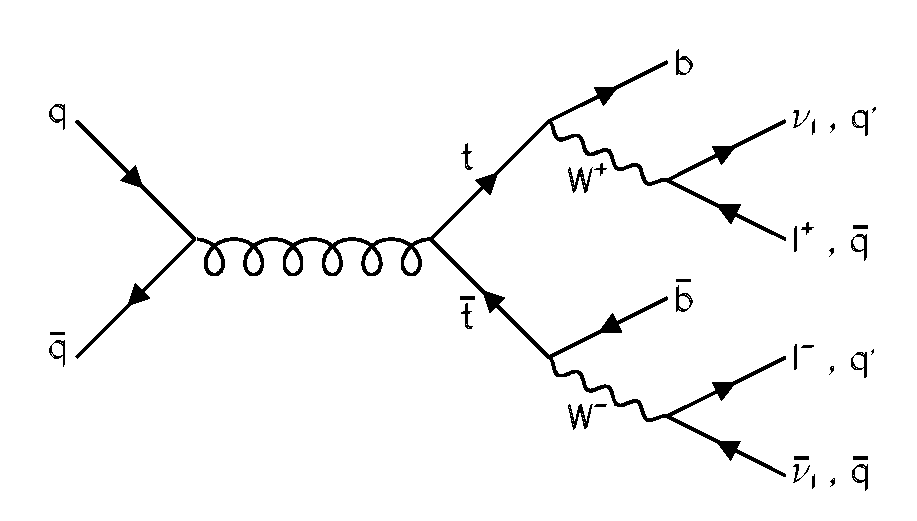
\includegraphics[width=\linewidth]{feynman/ttbar_decay.pdf}
    \end{minipage}
    \caption{Lowest order Feynman diagram for the production and decay a top anti-top quark pair from a gluon to a dilepton bottom anti-bottom system. \cite{PhysRevLett.79.3585}}
    \label{fig:ttbar-dilep}
\end{figure}
\begin{figure}
    \centering
    \begin{minipage}{0.4\textwidth}
        \centering
        \includegraphics[width=\linewidth]{plots/invar-mass_no-cut_ee_nt.png}
    \end{minipage}
    \caption{Plot of the invariant mass of $e^{+}e^{-}$ pair with only base physically motivated cuts. (electron pair with opposite charge).  Cuts derived from this was a lower and upper bound of $ -65\text{ GeV} < m_{ee} < 150 \text{ GeV}$}
    \label{fig:invar-mass_no-cut_ee}
\end{figure}
\begin{figure}
    \centering
    \begin{minipage}{0.4\textwidth}
        \centering
        \includegraphics[width=\linewidth]{plots/ptcone_ee_nt.png}
    \end{minipage}
    \caption{Plot of the ptcone30 of single electron (first lepton) with only base physically motivated cuts.  Cuts derived from this was an upper bound of $ptcone30[i] < 5.8 \text{ GeV for } i \in \left\{ 0,1 \right\}$}
    \label{fig:ptcone_ee}
\end{figure}
Other sources of background include lepton showers and Bremsstrahlung radiation.  Lepton showers are when a lepton emits of photon which then pair produces a lepton anti-lepton pair - typically electron-positron pair due to a lower rest mass. These electrons and positrons can proceed to emit photons or annihilate with another electron/positron to also produce another photon which can carry this process on until the photons emitted are less than the invariant mass of an electron-positron pair. Bremsstrahlung radiation is produced when a charged particle accelerates in an EM field resulting in photons being emitted. These photons can result in pair production occurring, therefore generating background. Both lepton showers and Bremsstrahlung radiation can be reduced by considering isolation variables, number of leptons, and the invariant mass of the system.
%%%%%%%%%%%%%%%%%%%%%%%%%%%%%%%%%% Analysis %%%%%%%%%%%%%%%%%%%%%%%%%%%%%%%%%%
\section{Analysis}
To select events most likely to correspond with $Z \rightarrow e^{+}e^{-}$, only events with two leptons, which are oppositely charged and of the type electron were used.

Using Eq.\ref{eq:invar-mass-2lep} and applying base physically motivated cuts, the invariant mass of electron-positron pairs were plotted on a stack plot to show the expected contribution of backgrounds and signal using the Monte Carlo (MC) data compmared to the experimental data from ATLAS.  This comparison is shown in Fig.\ref{fig:invar-mass_no-cut_ee}.

In addition to the invariant mass peak at $\sim 90 \text{ GeV}$ corresponding to the Z boson, there is a smaller peak at $\sim 10 \text{ GeV}$ attributed to the decay to upsilon ($b\bar{b}$) particles of mass $9.4 \text{ GeV}$\cite{10.2307-24955824}.
In the invariant mass range of $m_{ee} < 65 \text{ GeV}$ there is significant miss-modelling between the MC and ATLAS data. There is also a large amount of predicted background in this range.  Due to these two reasons, a lower bound of $m_{ee} > 65 \text{ GeV}$ was made. An upper bound of $m_{ee} < 150 \text{ GeV}$ was also made due to miss-modeling and increasing proportion of predicted background to signal.
% [h!]

In Fig.\ref{fig:ptcone_ee} the ptcone30 was plotted.  Due to limitations of the detector and detection techniques, no events less than 1 GeV are included in the detection.  This leads to a large peak at 0 GeV comprising of all events in the range $0 \text{ GeV} < ptcone < 1 \text{ GeV}$. Despite this, the MC models the general trend of the real data well upto 5.8 GeV.  However, the MC fails to predict the number of events suggesting an under estimation of background sources.  Since this effect is relatively uniform over this momentum range, this effect can not be used to motivate a cut. An upper bound of $ptcone30 < 5.8 \text{ GeV}$ was made due to greater miss-modelling. Since leptons produced by the decay of Z bosons tend to be relatively isolated, signal events would be expected to tend to have lower \textit{ptcone30} and \textit{etcone20}.   This further supports the cuts made.

The same process was also applied to \textit{etcone20} to motivate the bound of $-2 \text{ GeV} < etcone20 < 6 \text{ GeV}$ as shown in Fig.\ref{fig:etcone_ee}. Unlike \textit{ptcone30}, there are negative values for energy.  This arises from an over correction in an attempt to compensate for the ATLAS detector being less capable of reconstructing events with low energies. 

A lower bound was applied of $26 \text{ GeV} > p_T$ (Fig.\ref{fig:pt_ee}).  This was motivated be the miss-modeling between MC and experimental data.  Since the Z boson is expected to be produced almost at rest, the electron-positron pair is expected to be produced back to back with a high transverse momenta - further supporting a lower bound. Applying all cuts, the ATLAS data is well modelled in the invariant mass range of $60 \text{ GeV} < m_{ee} < 150 \text{ GeV}$ (Fig.\ref{fig:invar-mass_final-cuts_ee})

\begin{figure}
    \centering
    \begin{minipage}{0.4\textwidth}
        \centering
        \includegraphics[width=\linewidth]{plots/etcone_ee_nt.png}
    \end{minipage}
    \caption{Plot of the etcone20 of single electron (first lepton) with only base physically motivated cuts. Cuts derived from this was a lower and upper bound of $ -2\text{ GeV} < etcone20[i] < 6 \text{ GeV for } i \in \left\{ 0,1 \right\}$}
    \label{fig:etcone_ee}
\end{figure}
\begin{figure}
    \centering
    \begin{minipage}{0.4\textwidth}
        \centering
        \includegraphics[width=\linewidth]{plots/pT_ee_nt.png}
    \end{minipage}
    \caption{Plot of the transverse momentum of individual electron with only base physically motivated cuts. (electron pair with opposite charge).  Cuts derived from this was a lower and upper bound of $ -2\text{ GeV} < etcone20[i] < 6 \text{ GeV for } i \in \left\{ 0,1 \right\}$}
    \label{fig:pt_ee}
\end{figure}
\begin{figure}
    \centering
    \begin{minipage}{0.4\textwidth}
        \centering
        \includegraphics[width=\linewidth]{plots/invar-mass_full-cut_ee_nt.png}
    \end{minipage}
    \caption{Plot of the invariant mass of electron-positron pair with the final cuts applied. (electron pair with opposite charge)}
    \label{fig:invar-mass_final-cuts_ee}
\end{figure}
%%%%%%%%%%%%%%%%%%%%%%%%%%%%%%%%%% Results %%%%%%%%%%%%%%%%%%%%%%%%%%%%%%%%%%
\section{Results}
Using Eq.\ref{eq:cs} the cross section was found to be $\sigma (pp \rightarrow Z \rightarrow ) = 1.988\pm0.001 (\text{stat.}) \pm 0.136 (\text{syst.}) \pm 0.0338 (\text{lumi.}) \text{ nb}$. $N^{background}$ was estimated to be the sum of weights of MC events which pass the selection cuts. The main source of background was t-tbar. $\epsilon$ was estimated to be the ratio between the sum of weights of MC events which pass the cuts and the sum of weights for all MC signal events.

The uncertainty is split into three main contributions: statistical, systematic, and luminosity. To estimate the statistical contribution, the counting approximation was used on each value to give $\sqrt{N}$ where $N$ is the number of events. To estimate the systematic contributions, each cut was varied independently and half of the range was taken to be the contribution from that cut. This was repeated for each cut and then added in quadrature. 
%%%%%%%%%%%%%%%%%%%%%%%%%%%%%%%%%% Conclusion %%%%%%%%%%%%%%%%%%%%%%%%%%%%%%%%%%
\section{Conclusion}
The cross section $\sigma (pp \rightarrow Z \rightarrow ) = 1.988\pm0.001 (\text{stat.}) \pm 0.136 (\text{syst.}) \pm 0.0338 (\text{lumi.}) \text{ nb}$ was found by comparing experimental data and Monte Carlo simulations to suggest selection cuts to reduce background.  The main source of error was the systematic uncertainty. Improvements could have been made on the estimation of background events by using experimental not MC data.

% \nocite{*}
\bibliography{main}

\end{document}
